% Presentation on keg
%
\documentclass{beamer}
%\documentclass[handout]{beamer}
%\usepackage{beamerthemeshadow}
\usetheme{Warsaw}
\usepackage{pgf}
\usepackage{multimedia}

%\pgfdeclareimage[interpolate=true,height=7cm]{faktorial}{faktorial}

\author{Michal Kov\'{a}\v{c}}
\title{User oriented language for powerful data mining with Ferda}
\date{\today}

\begin{document}
\frame{\titlepage}

\section{Introduction}
\subsection{Table of contents}
\frame{
	\frametitle{Table of contents part 1/2}
	\tableofcontents[sections={1-2},pausesections]
}

\frame{
	\frametitle{Table of contents part 2/2}
	\tableofcontents[sections={3-4},pausesections]
}

\subsection{What is Ferda Data Miner?}
\begin{frame}
	\frametitle{Ferda}
	\begin{block}{What is Ferda?}
		\begin{itemize}[<+->]
			\item User oriented application
			\item For specification of tasks, execution and result browsing
			\item Works with boxes
			\item Ferda Data Miner = Ferda + boxes for data mining
		\end{itemize}
	\end{block}
	\begin{block}<+->{History}
		\begin{itemize}[<+->]
			\item LISp-Miner not so much user frienly
			\item Software project at MFF
			\item Diploma theses
		\end{itemize}
	\end{block}
\end{frame}

\begin{frame}
	\frametitle{Screenshot}
	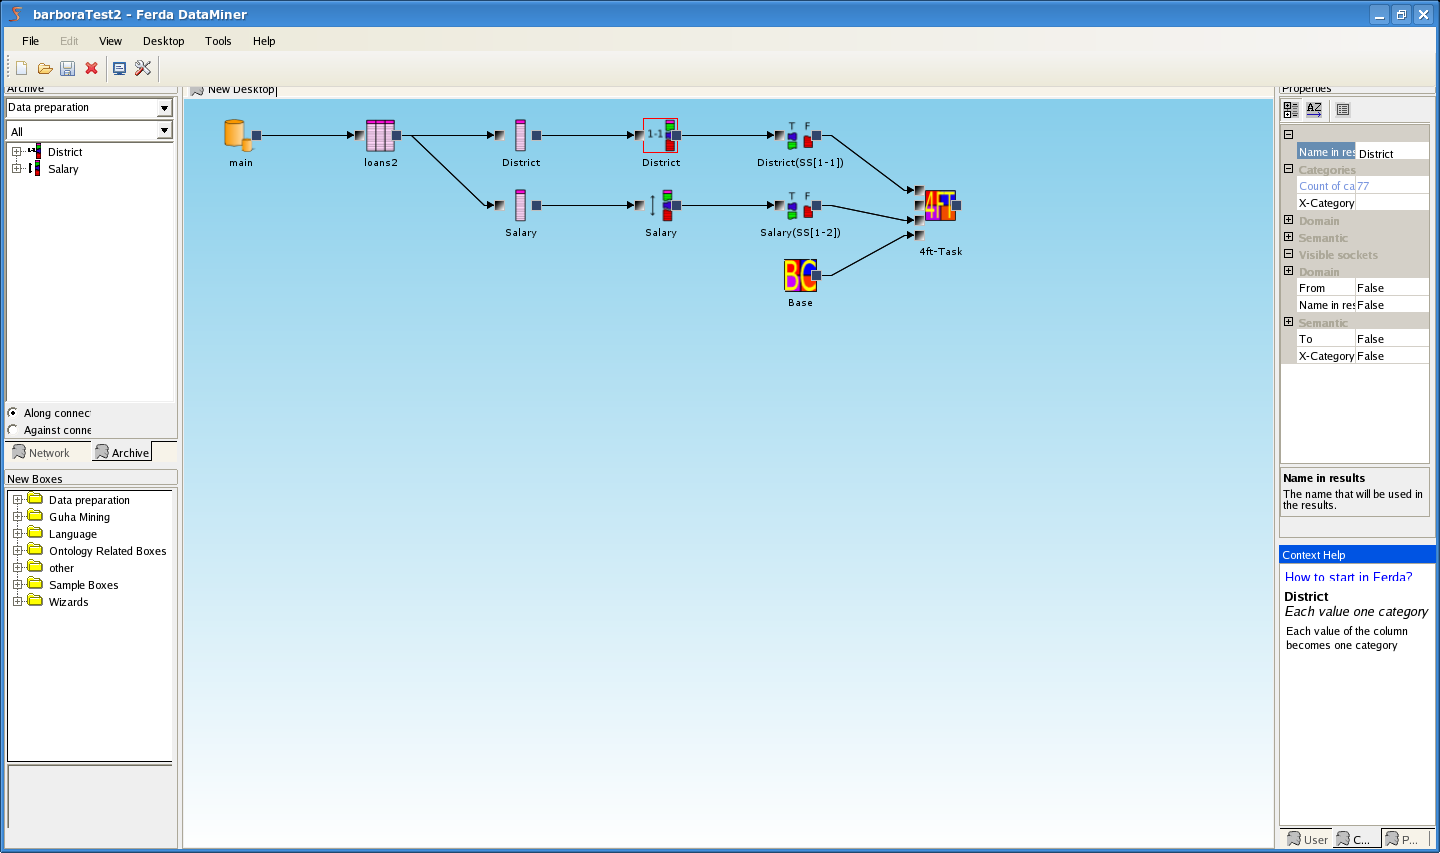
\includegraphics[width=10.8cm]{ferda}
\end{frame}

\subsection{Ferda as programming language}
\begin{frame}
	\frametitle{Ferda as programming language}
	\begin{block}<+->{Box as function}
		\begin{itemize}[<+->]
			\item Box consists of function
			\item Socket is parameter of ths function
			\item Property is also socket
				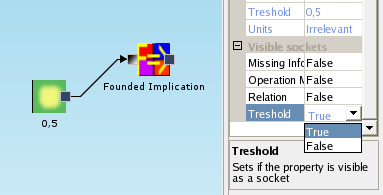
\includegraphics[width=7cm]{property_as_socket}
		\end{itemize}
	\end{block}	
\end{frame}

\subsection{What is missing? What should be done?}
\begin{frame}
	\frametitle{What is missing?}
	\begin{block}{What is missing?}
		\begin{itemize}[<+->]
			\item Moving work from one project to another
			\item Basic math boxes
			\item Recursion
			\item Other language boxes
			\item Ferda specific language boxes
			\item Data mining specific boxes for user programming
		\end{itemize}
	\end{block}
\end{frame}

\section{New functionality in Ferda}
\subsection{Network archive}
\begin{frame}
	\frametitle{Network archive}
	\begin{block}{What is network archive?}
		\begin{itemize}[<+->]
			\item New place where user can store connection
			\item Independent on project
			\item One network archive can be used from more computers
			\item Way how to move connections from one project to another
		\end{itemize}
	\end{block}
\end{frame}

\begin{frame}
	\frametitle{Movie -- network archive}
	\movie[externalviewer]{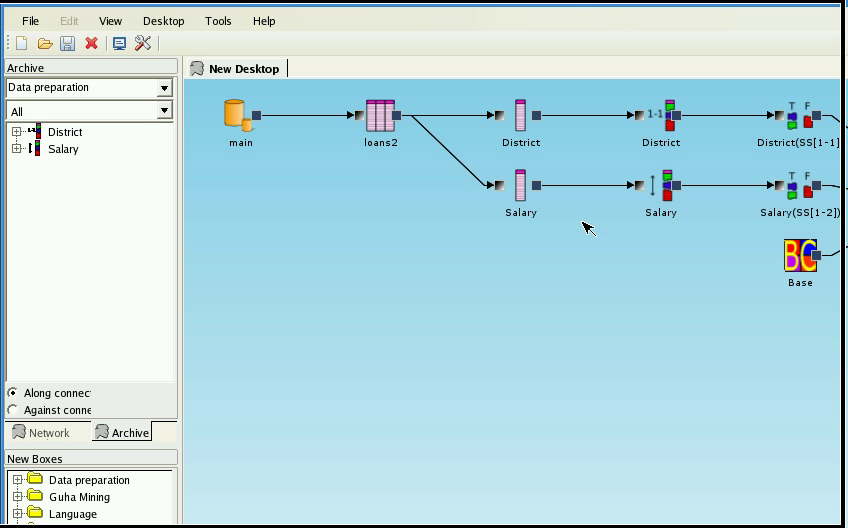
\includegraphics[width=10.8cm]{networkArchive1}}{networkArchive.ogg}
\end{frame}

\begin{frame}
	\frametitle{Screenshot -- add a connection to the network archive}
	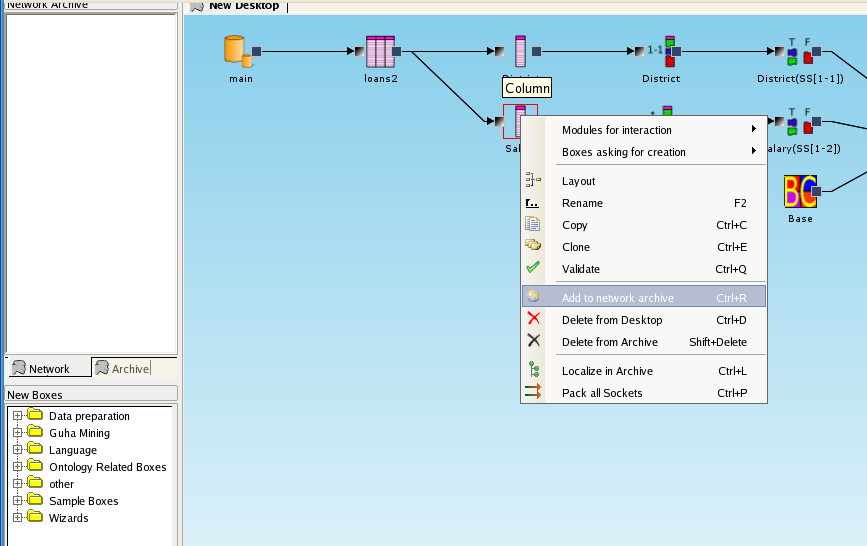
\includegraphics[width=10.8cm]{add_to_network_archive}
\end{frame}

\begin{frame}
	\frametitle{Screenshot -- set a name of box in the network archive}
	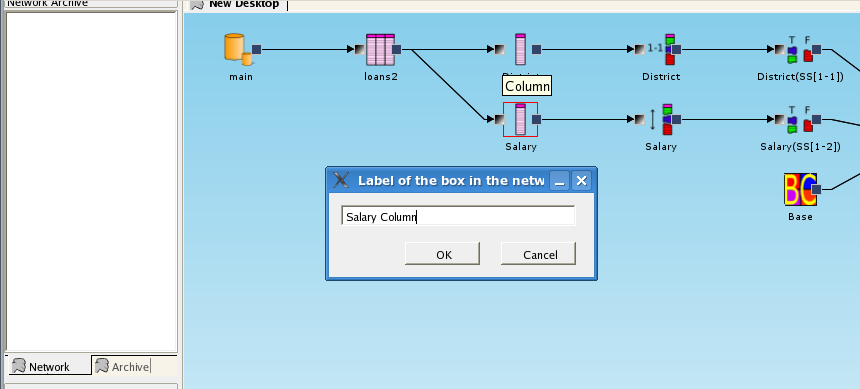
\includegraphics[width=10.8cm]{set_name_of_box_in_network_archive}
\end{frame}

\begin{frame}
	\frametitle{Screenshot -- new box added to the network archive}
	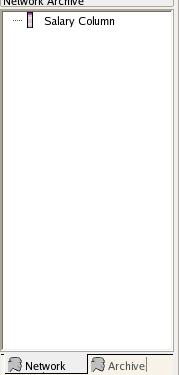
\includegraphics[height=7cm]{network_archive_box_added}
\end{frame}

\begin{frame}
	\frametitle{Screenshot -- drop box to a desktop from the n. archive}
	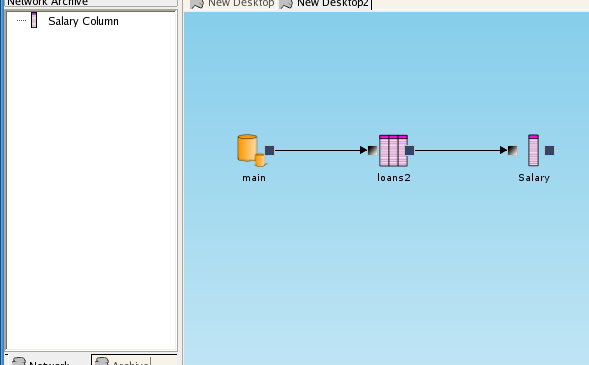
\includegraphics[width=10.8cm]{network_archive_drop_to_desktop}
\end{frame}

\begin{frame}
	\frametitle{Screenshot -- remove box from the network archive}
	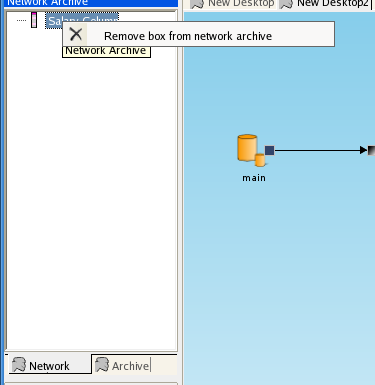
\includegraphics[height=7cm]{network_archive_remove_box}
\end{frame}

\subsection{Boxes for math}
\begin{frame}
	\frametitle{Movie -- Binary operation}
	\movie[externalviewer]{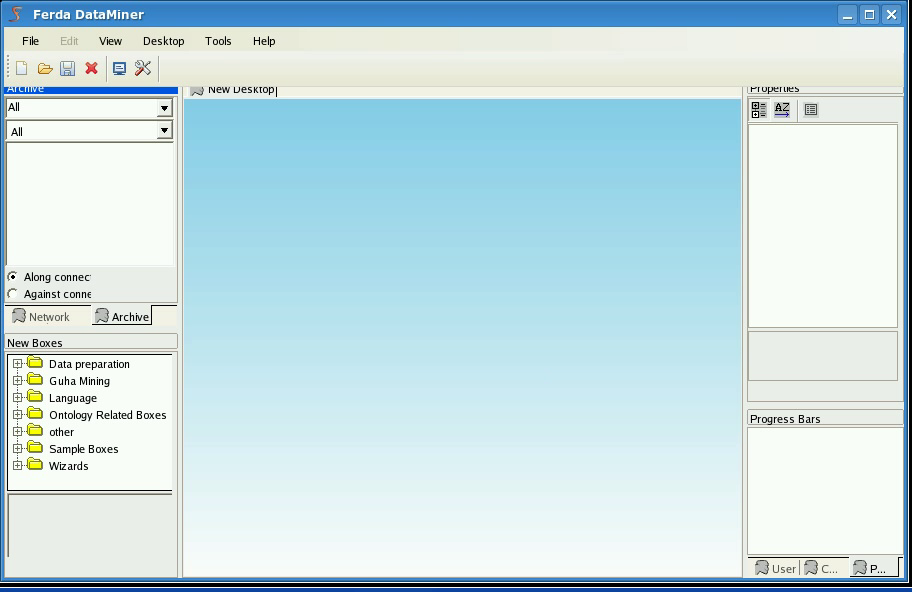
\includegraphics[width=10.8cm]{binaryOperation1.png}}{binaryOperation.ogg}
\end{frame}

\begin{frame}
	\frametitle{Binary operation}
	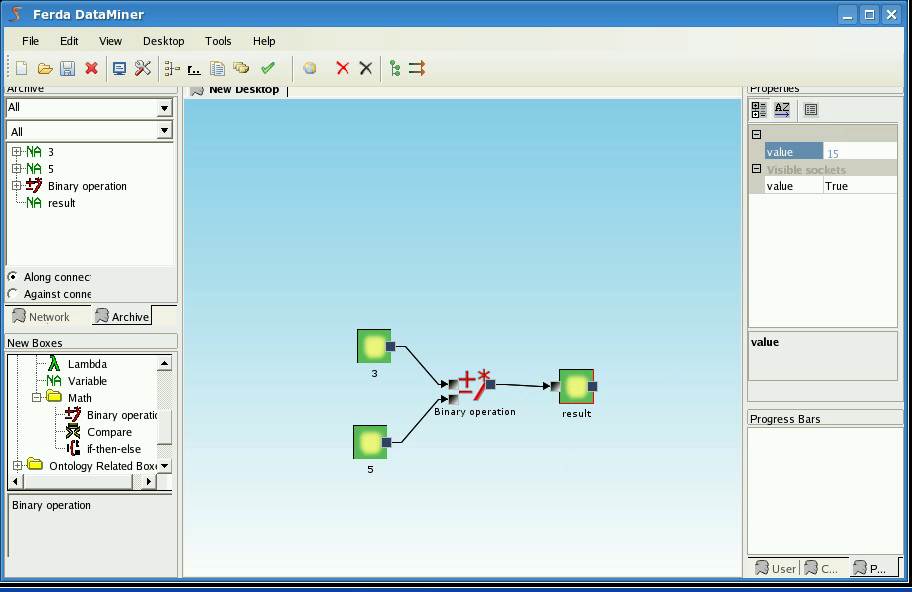
\includegraphics[width=10.8cm]{binaryOperation2.png}
\end{frame}

\begin{frame}
	\frametitle{Movie -- Comparision}
	\movie[externalviewer]{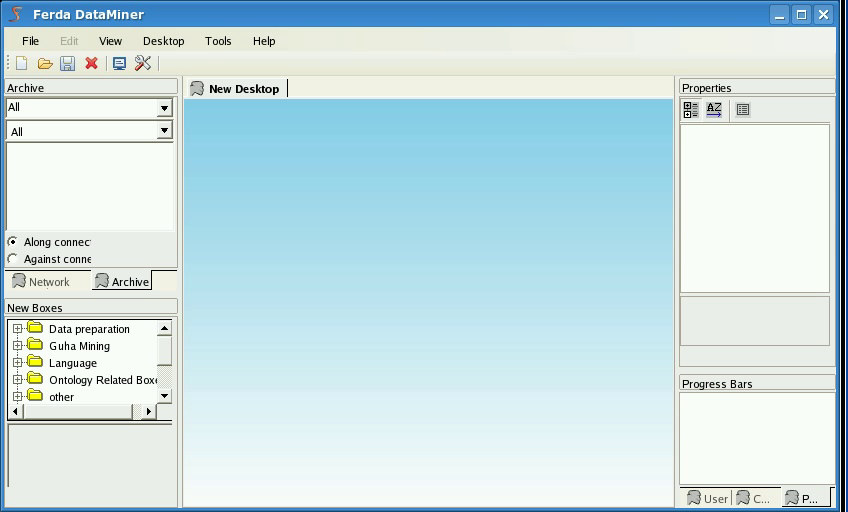
\includegraphics[width=10.8cm]{compare1.png}}{compare.ogg}
\end{frame}

\begin{frame}
	\frametitle{Comparision}
	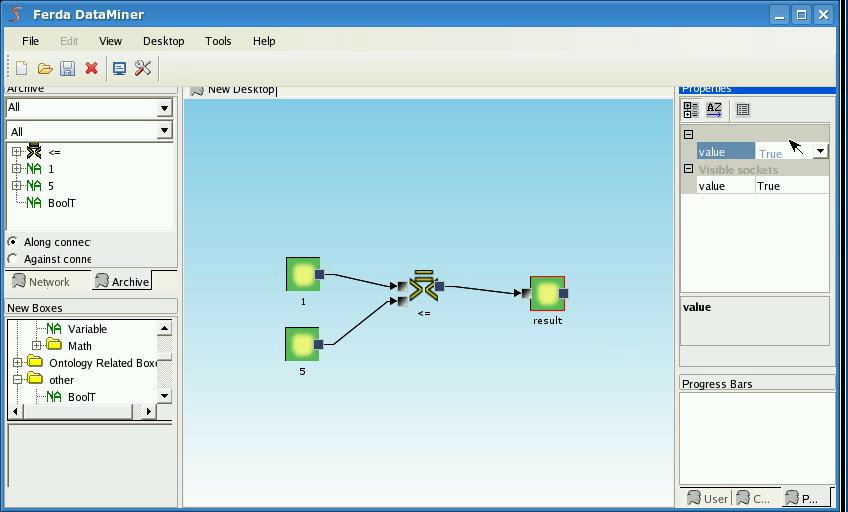
\includegraphics[width=10.8cm]{compare2.png}
\end{frame}

\begin{frame}
	\frametitle{Movie -- If expression}
	\movie[externalviewer]{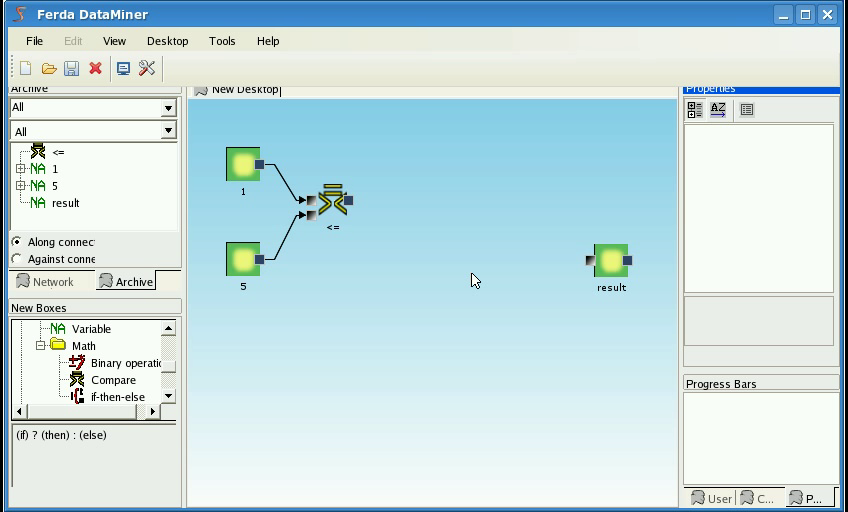
\includegraphics[width=10.8cm]{ifthenelse1.png}}{ifthenelse.ogg}
\end{frame}

\begin{frame}
	\frametitle{If expressions}
	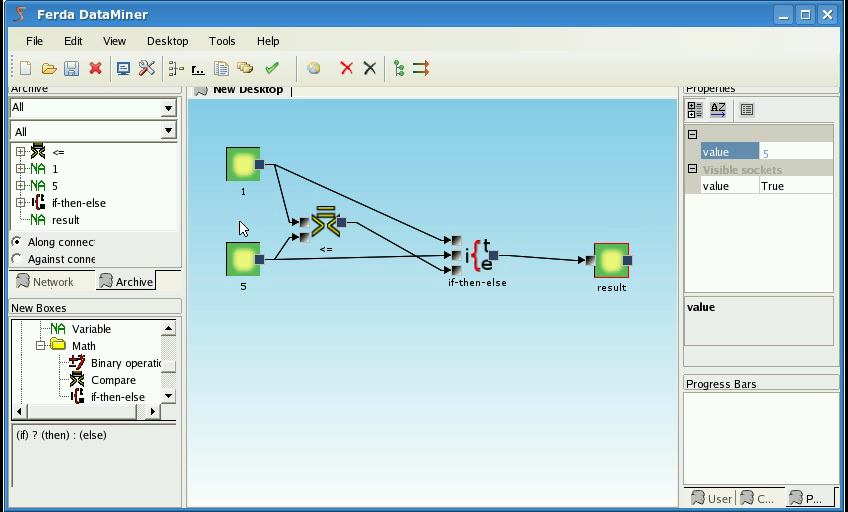
\includegraphics[width=10.8cm]{ifthenelse2.png}
\end{frame}

\subsection{Lambda function}
\begin{frame}
	\frametitle{Lambda in other languages}
\end{frame}

\begin{frame}
	\frametitle{Movie -- Lambda basics in Ferda}
	\movie[externalviewer]{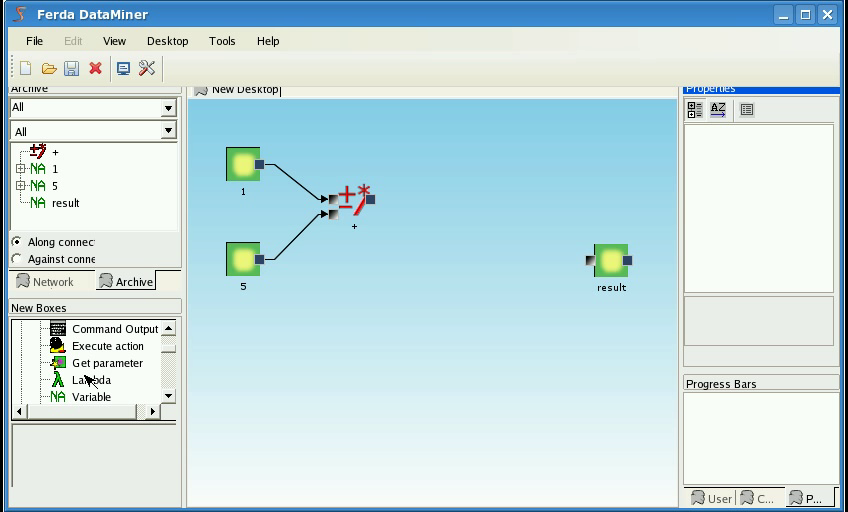
\includegraphics[width=10.8cm]{lambdaBasic1.png}}{lambdaBasic.ogg}
\end{frame}

\begin{frame}
	\frametitle{Basic use in Ferda}
	\framesubtitle{Lambda without parameters}

	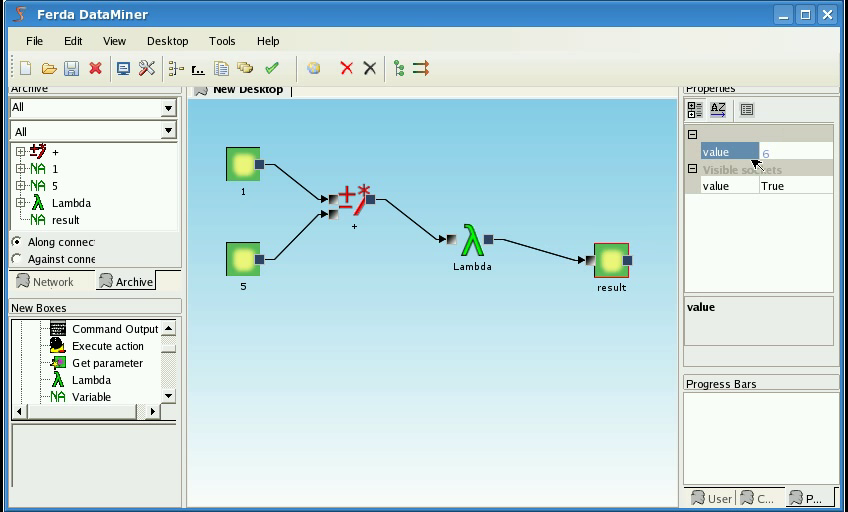
\includegraphics[width=10.8cm]{lambdaBasic2.png}
\end{frame}

\begin{frame}
	\frametitle{Basic use in Ferda}
	\framesubtitle{One constant parameter specified}
	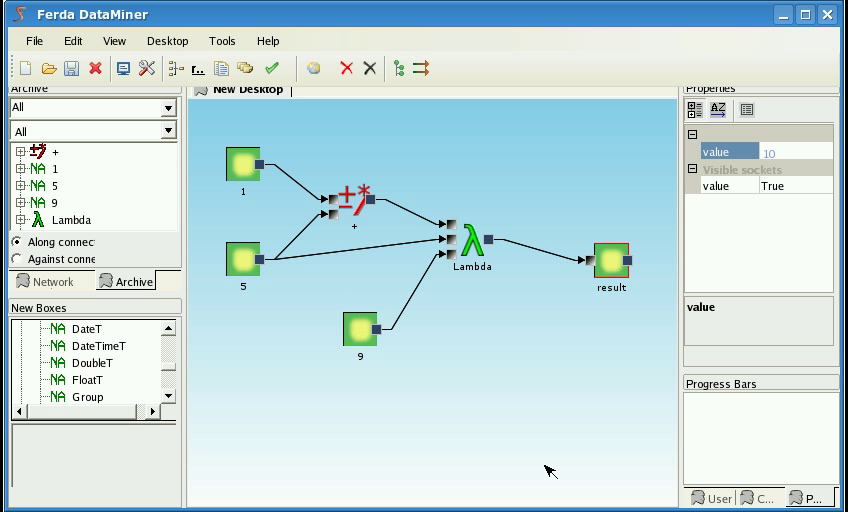
\includegraphics[width=10.8cm]{lambdaBasic3.png}
\end{frame}

\begin{frame}[fragile]
	\frametitle{Factorial in C\#}
	\framesubtitle{Structural version}

	\begin{block}{First version of factorial}
\begin{verbatim}
public static int Factorial(int x)
{
  if (x == 0)
  {
    return 1;
  }
  else
  {
    return x * Factorial(x - 1);
  }
}
\end{verbatim}
	\end{block}
\end{frame}

\begin{frame}[fragile]
	\frametitle{Factorial in C\#}
	\framesubtitle{Expresion version}

	\begin{block}{Second version of factorial}
\begin{verbatim}
public static int Factorial2(int x)
{
  return (x == 0) ? 1 : x * Factorial2(x - 1);
}
\end{verbatim}
	\end{block}
\end{frame}

\begin{frame}[fragile]
        \frametitle{Factorial in other languages}

	\begin{block}<+->{Python}
\begin{verbatim}
l = lambda x: x == 0 and 1 or x * factorial(x - 1)
\end{verbatim}
	\end{block}

	\begin{block}<+->{F\#}
\begin{verbatim}
let rec factorial n =
    if n=0 then 1 else n * factorial(n - 1)
\end{verbatim}
	\end{block}
\end{frame}

\begin{frame}
	\frametitle{Factorial in Ferda}
	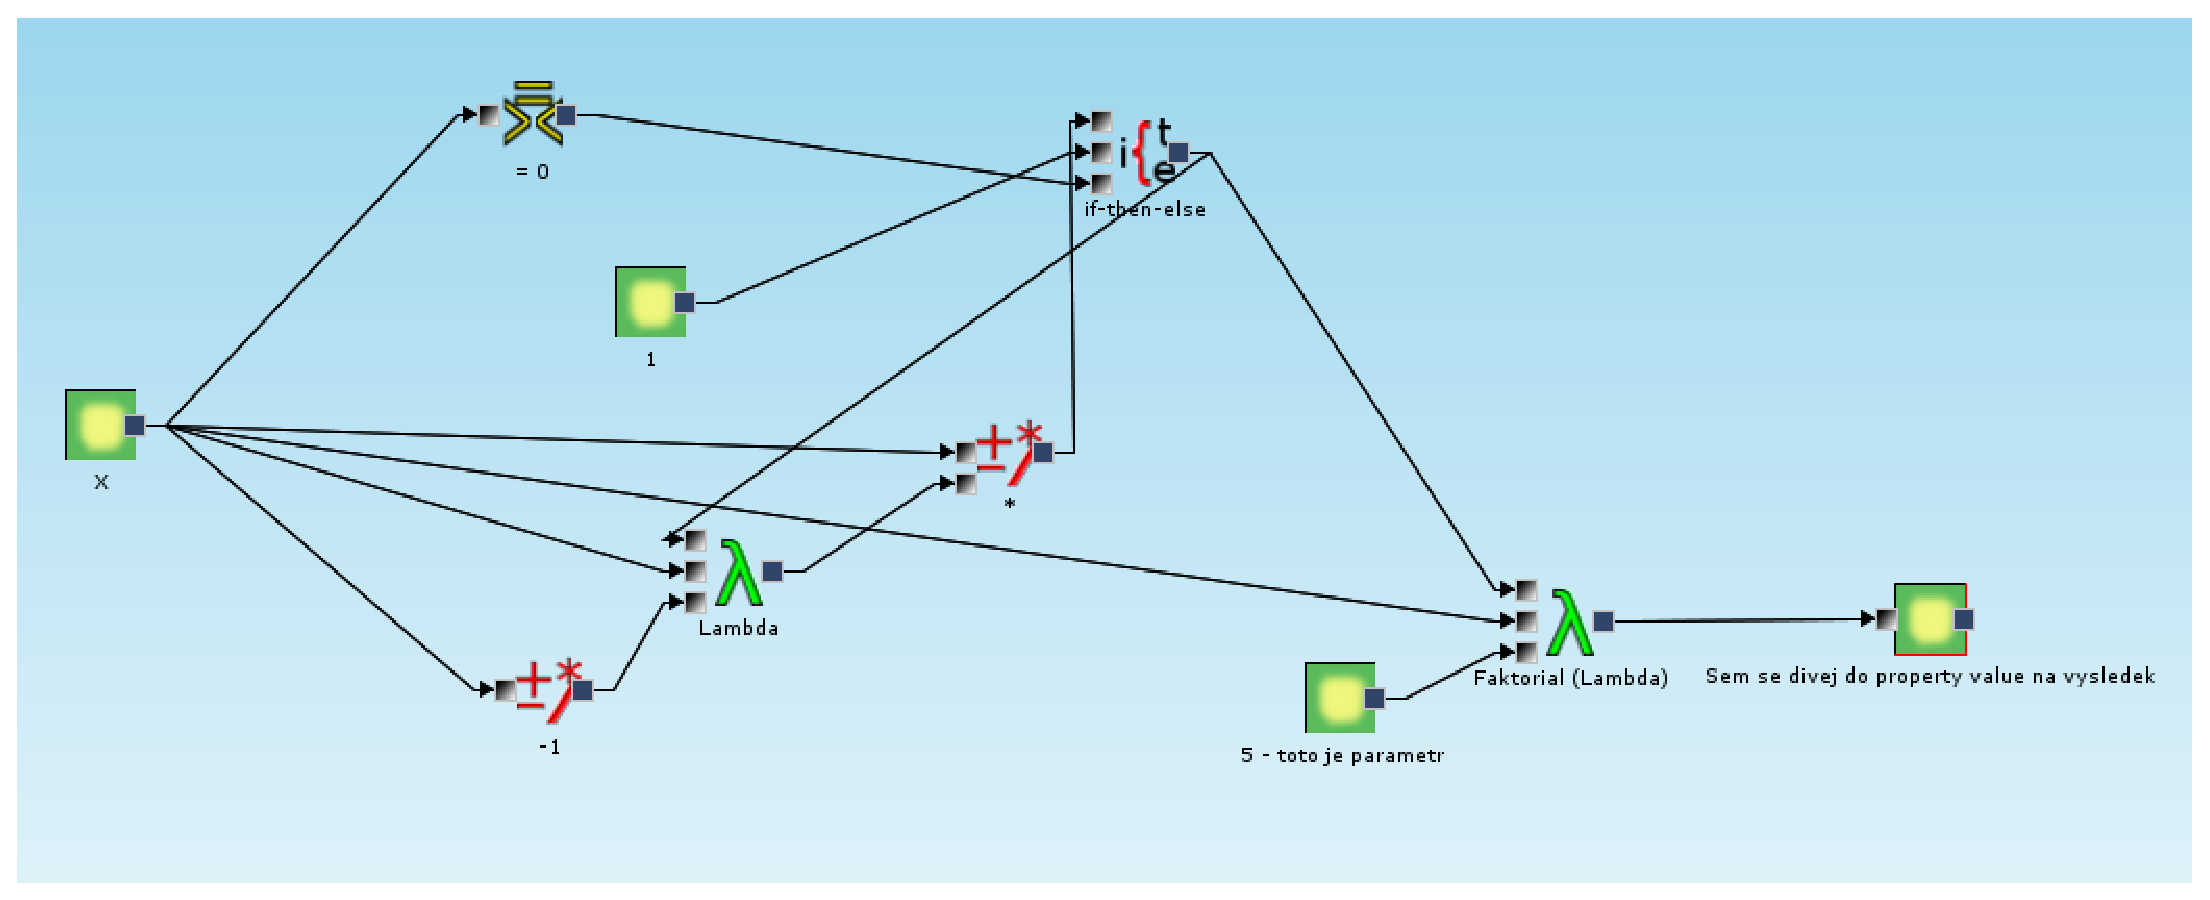
\includegraphics[width=10.8cm]{faktorial}
\end{frame}

\subsection{Other new boxes}
\begin{frame}
	\frametitle{Movie -- Get parameter}
	\movie[externalviewer]{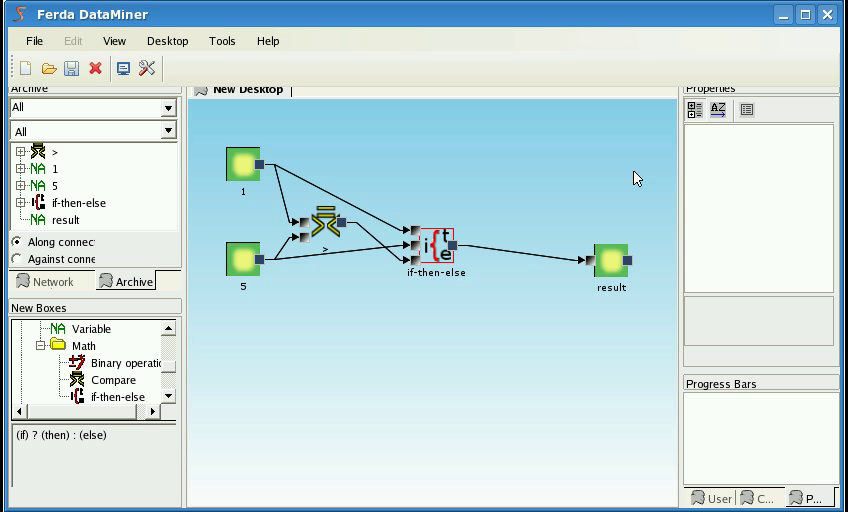
\includegraphics[width=10.8cm]{getParameter1.png}}{getParameter.ogg}
\end{frame}

\begin{frame}
	\frametitle{Get parameter}
	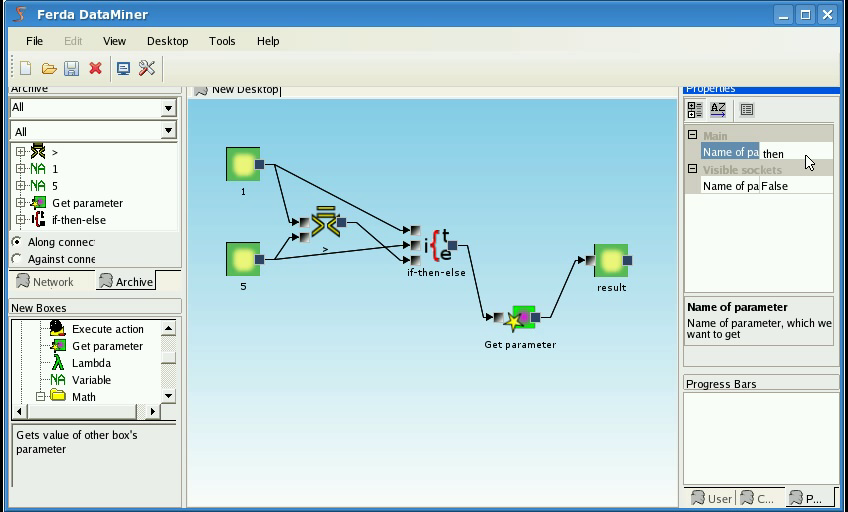
\includegraphics[width=10.8cm]{getParameter2.png}
\end{frame}

\begin{frame}
	\frametitle{Movie -- Execute action}
	\movie[externalviewer]{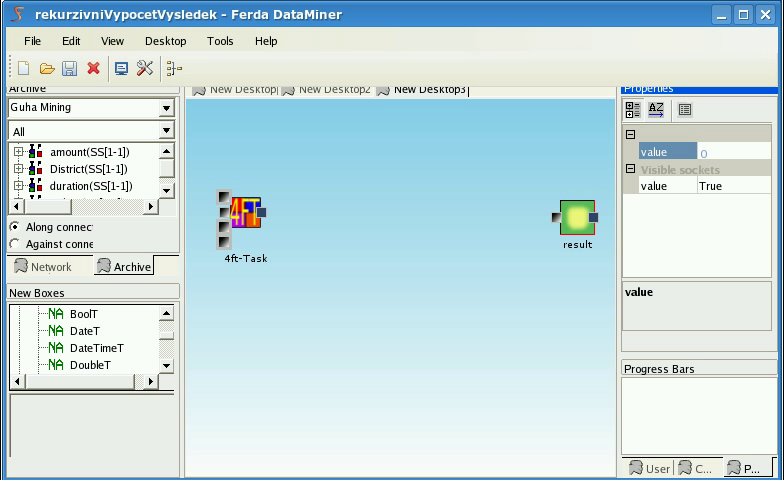
\includegraphics[width=10.8cm]{executeAction1.png}}{executeAction.ogg}
\end{frame}

\begin{frame}
	\frametitle{Execute action}
	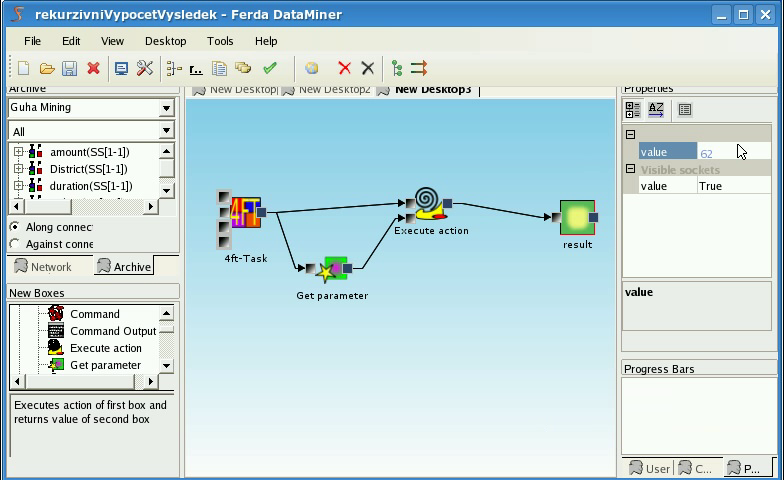
\includegraphics[width=10.8cm]{executeAction2.png}
\end{frame}

\begin{frame}
	\frametitle{Movie -- Command and command output}
	\movie[externalviewer]{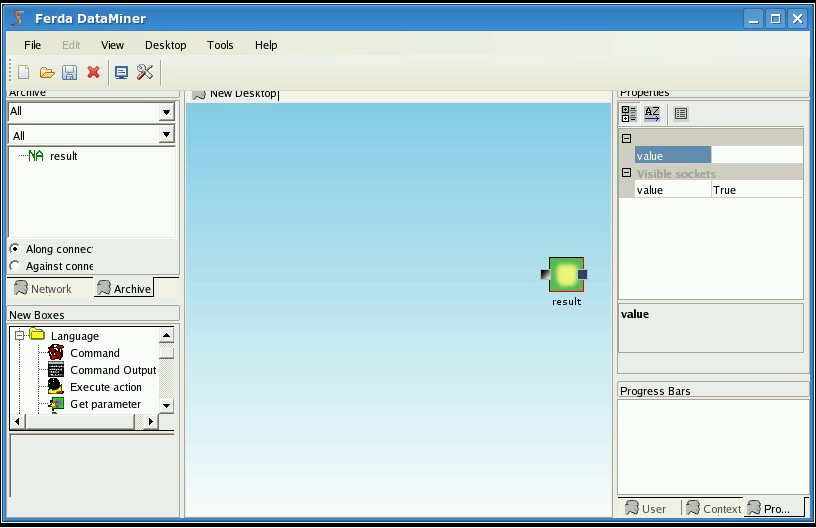
\includegraphics[width=10.8cm]{command1.png}}{command.ogg}
\end{frame}

\begin{frame}
	\frametitle{Command and command output}
	\framesubtitle{Example in ferda}
	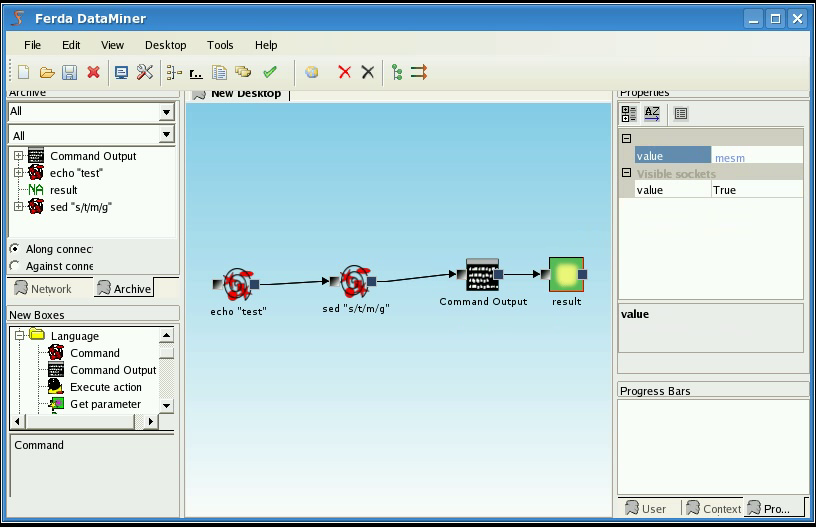
\includegraphics[width=10.8cm]{command2.png}
\end{frame}

\begin{frame}
	\frametitle{Command and command output}
	\subtitle{The same in console}
	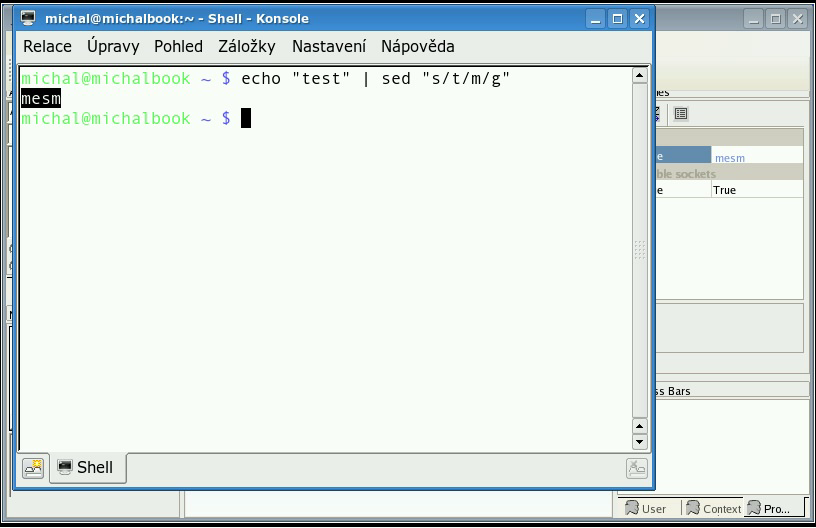
\includegraphics[width=10.8cm]{command3.png}
\end{frame}

\section{Example -- executing four fold task recursively}
\subsection{Motivation}
\begin{frame}
	\frametitle{Movie -- Motivation on basic four fold task}
	\movie[externalviewer]{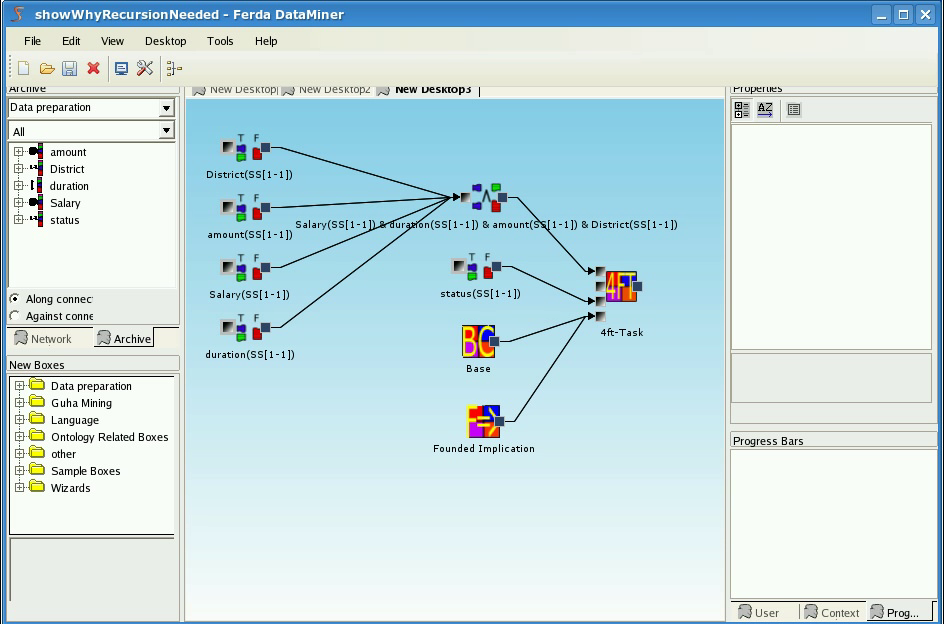
\includegraphics[width=10.8cm]{exampleMotivation1}}{exampleMotivation.ogg}
\end{frame}

\begin{frame}
	\frametitle{Motivation on basic four fold task}
	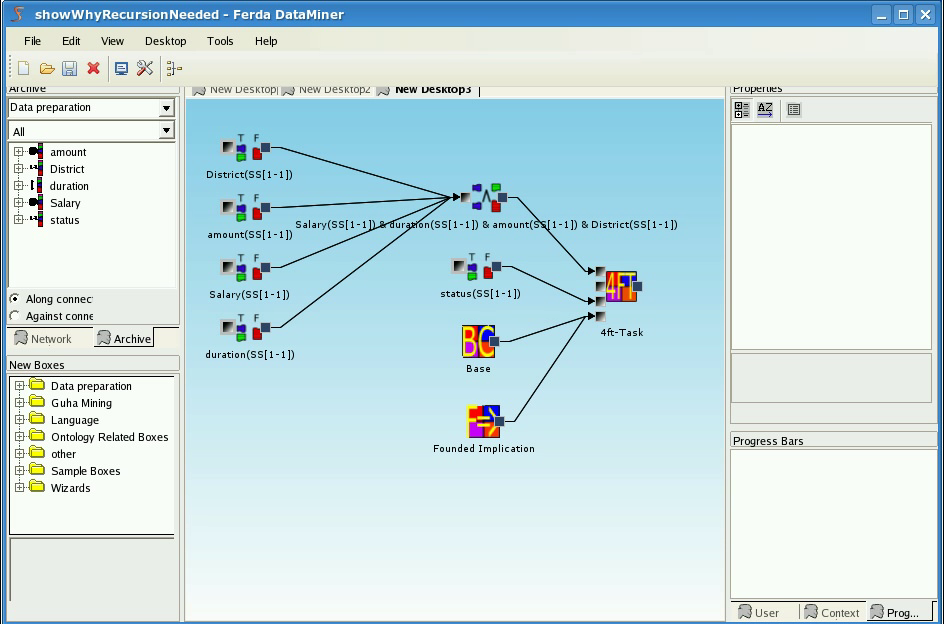
\includegraphics[width=5cm]{exampleMotivation1}
	\begin{block}<+->{Problem}
	\end{block}
\end{frame}

\begin{frame}
	\frametitle{User specified automation of settings}
\end{frame}

\subsection{Linear interpolation}
\begin{frame}
	\frametitle{Basics}
\end{frame}

\begin{frame}
	\frametitle{Interpolation as connection of boxes}
	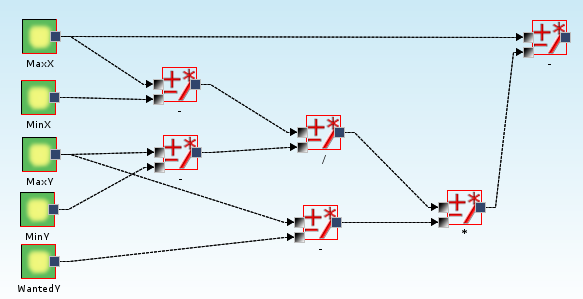
\includegraphics[width=10.8cm]{linearInterpolation}
\end{frame}

\subsection{Connection of boxes}
\begin{frame}
	\frametitle{Result should be between}
	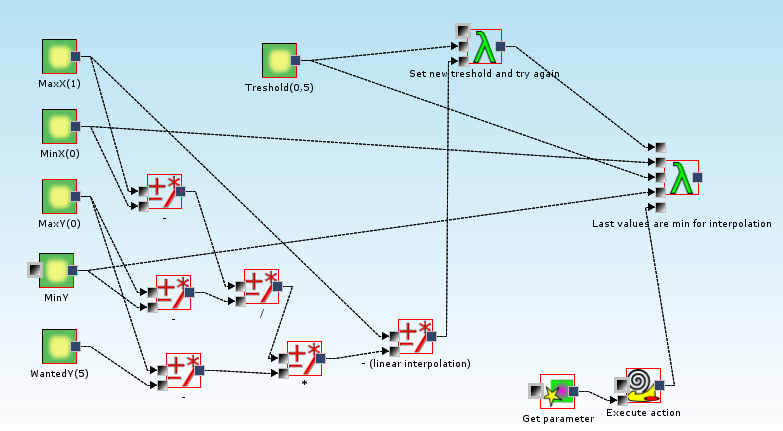
\includegraphics[width=10.8cm]{exampleMainRecursionPart}
\end{frame}

\begin{frame}
	\frametitle{If not interpolate and set new max/min}
	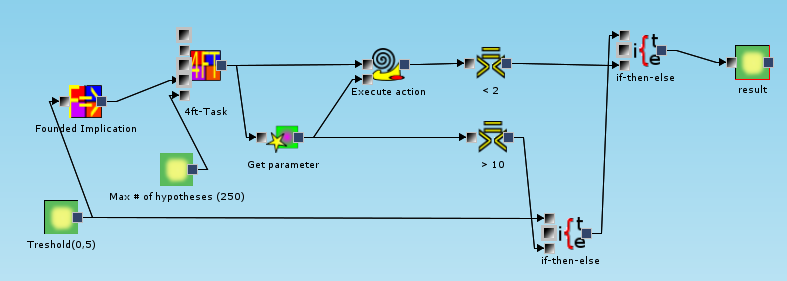
\includegraphics[width=10.8cm]{exampleMainMiningPart}
\end{frame}

\begin{frame}
	\frametitle{}
	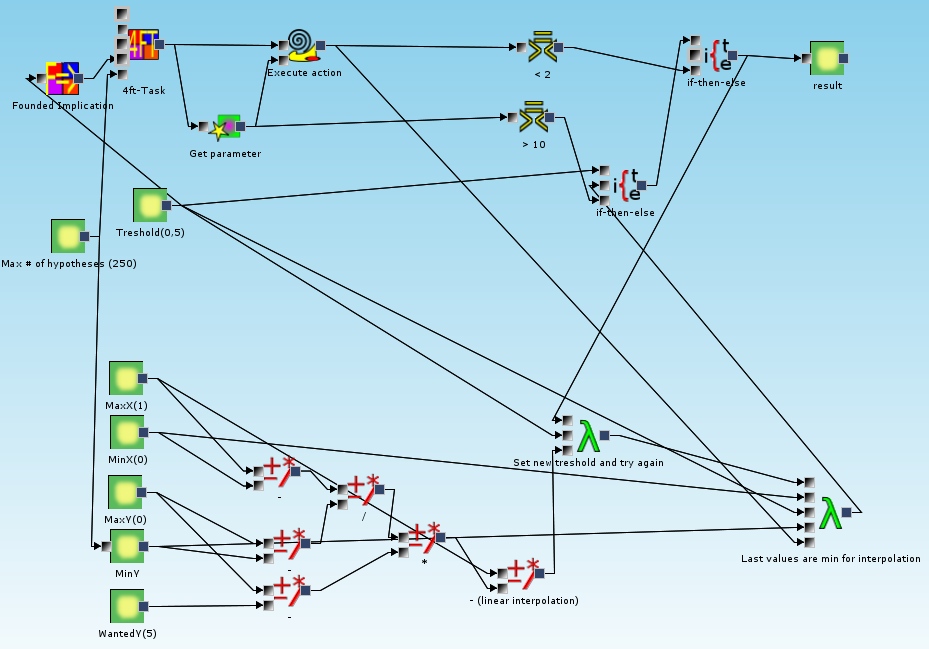
\includegraphics[width=10.8cm]{exampleWithoutInterpolationOnMax}
\end{frame}

\subsection{Results}
\begin{frame}
	\frametitle{Connection}
	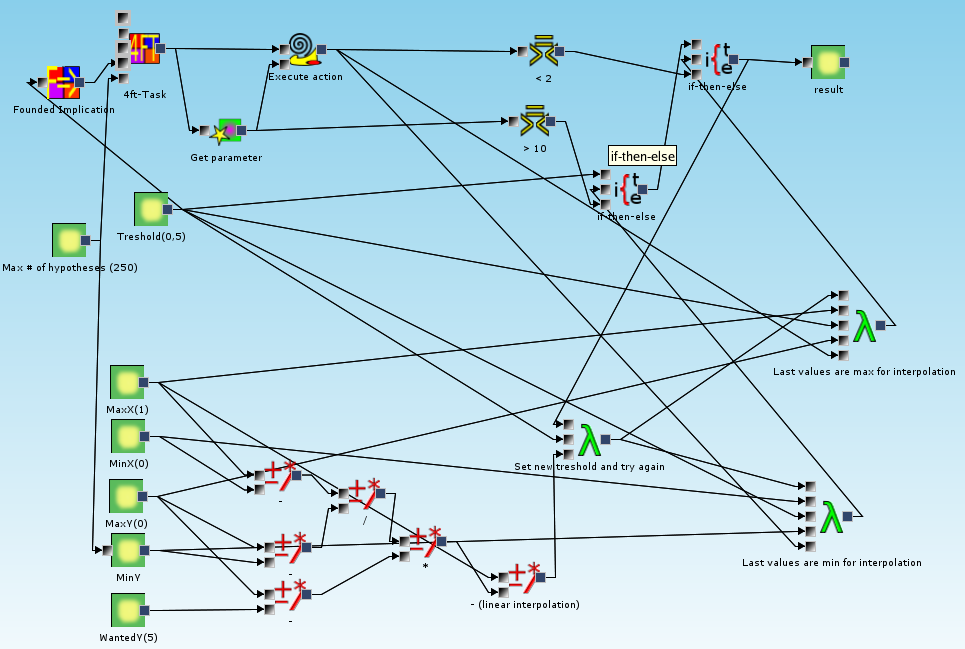
\includegraphics[width=10.8cm]{exampleResult}
\end{frame}

\begin{frame}
	\frametitle{Movie -- Result}
	\movie[externalviewer]{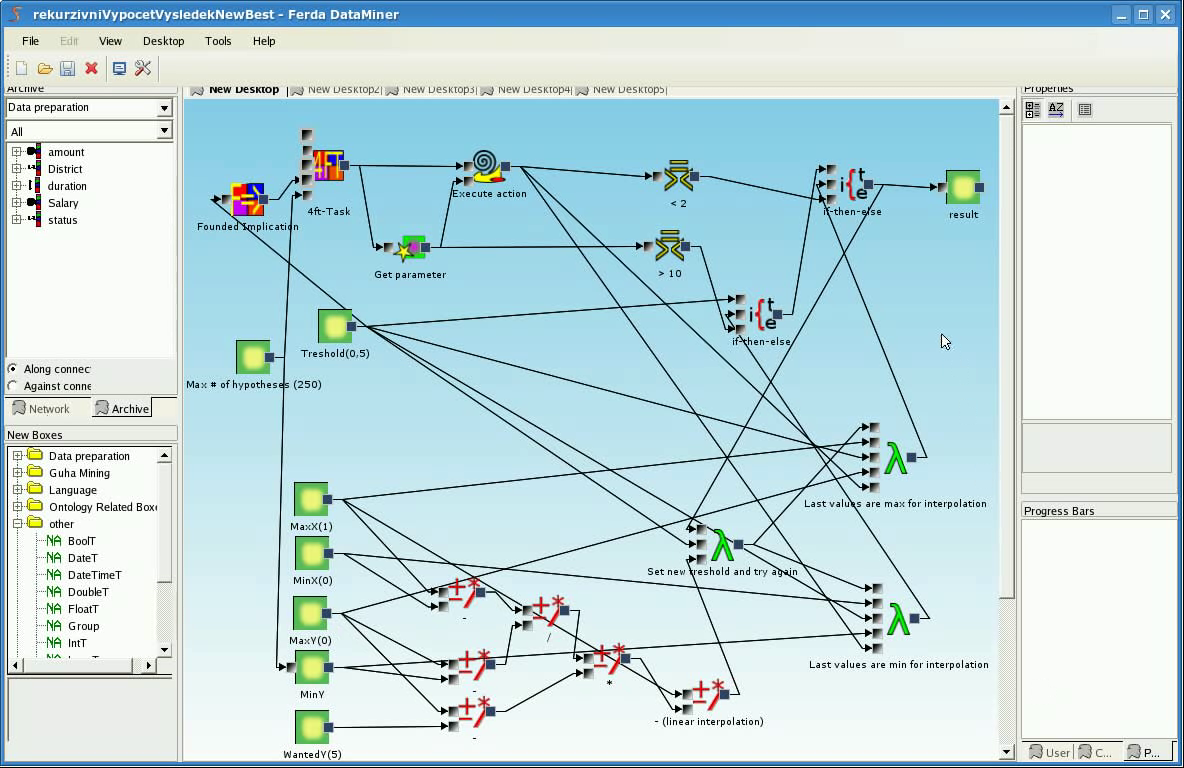
\includegraphics[width=10.8cm]{recursionExecution1}}{recursionExecution.ogg}
\end{frame}

\begin{frame}
	\frametitle{How to do it better}
%nepocitat zbytecne dokola
%bestn

\end{frame}

\section{Next steps}
\subsection{Sequences and sets}
\subsection{Reuse of code}
% includy, lepsi sitovy archiv, nahrani krabicek z jineho projektu

\subsection{Better lambda}

%dalsi:
% uzivatel si vybira, kde krabicka bezi
% moduly pro interakci nad skutecnym functions
\subsection{Summary}
\frame{vitez}

\end{document}
